\subsection{\eu Architecture}
\label{sec:europa:arch}

\eu is implemented as a library that encapsulates all the elements
described above and makes them easily accessible through modeling and
API layers.  A user will typically use the modeling facilities to
inject a problem domain description, and the API to extract and
manipulate plans, and to obtain information about plan flaws and
constraint violations at any stage of the planning process.

\begin{figure}
\centering
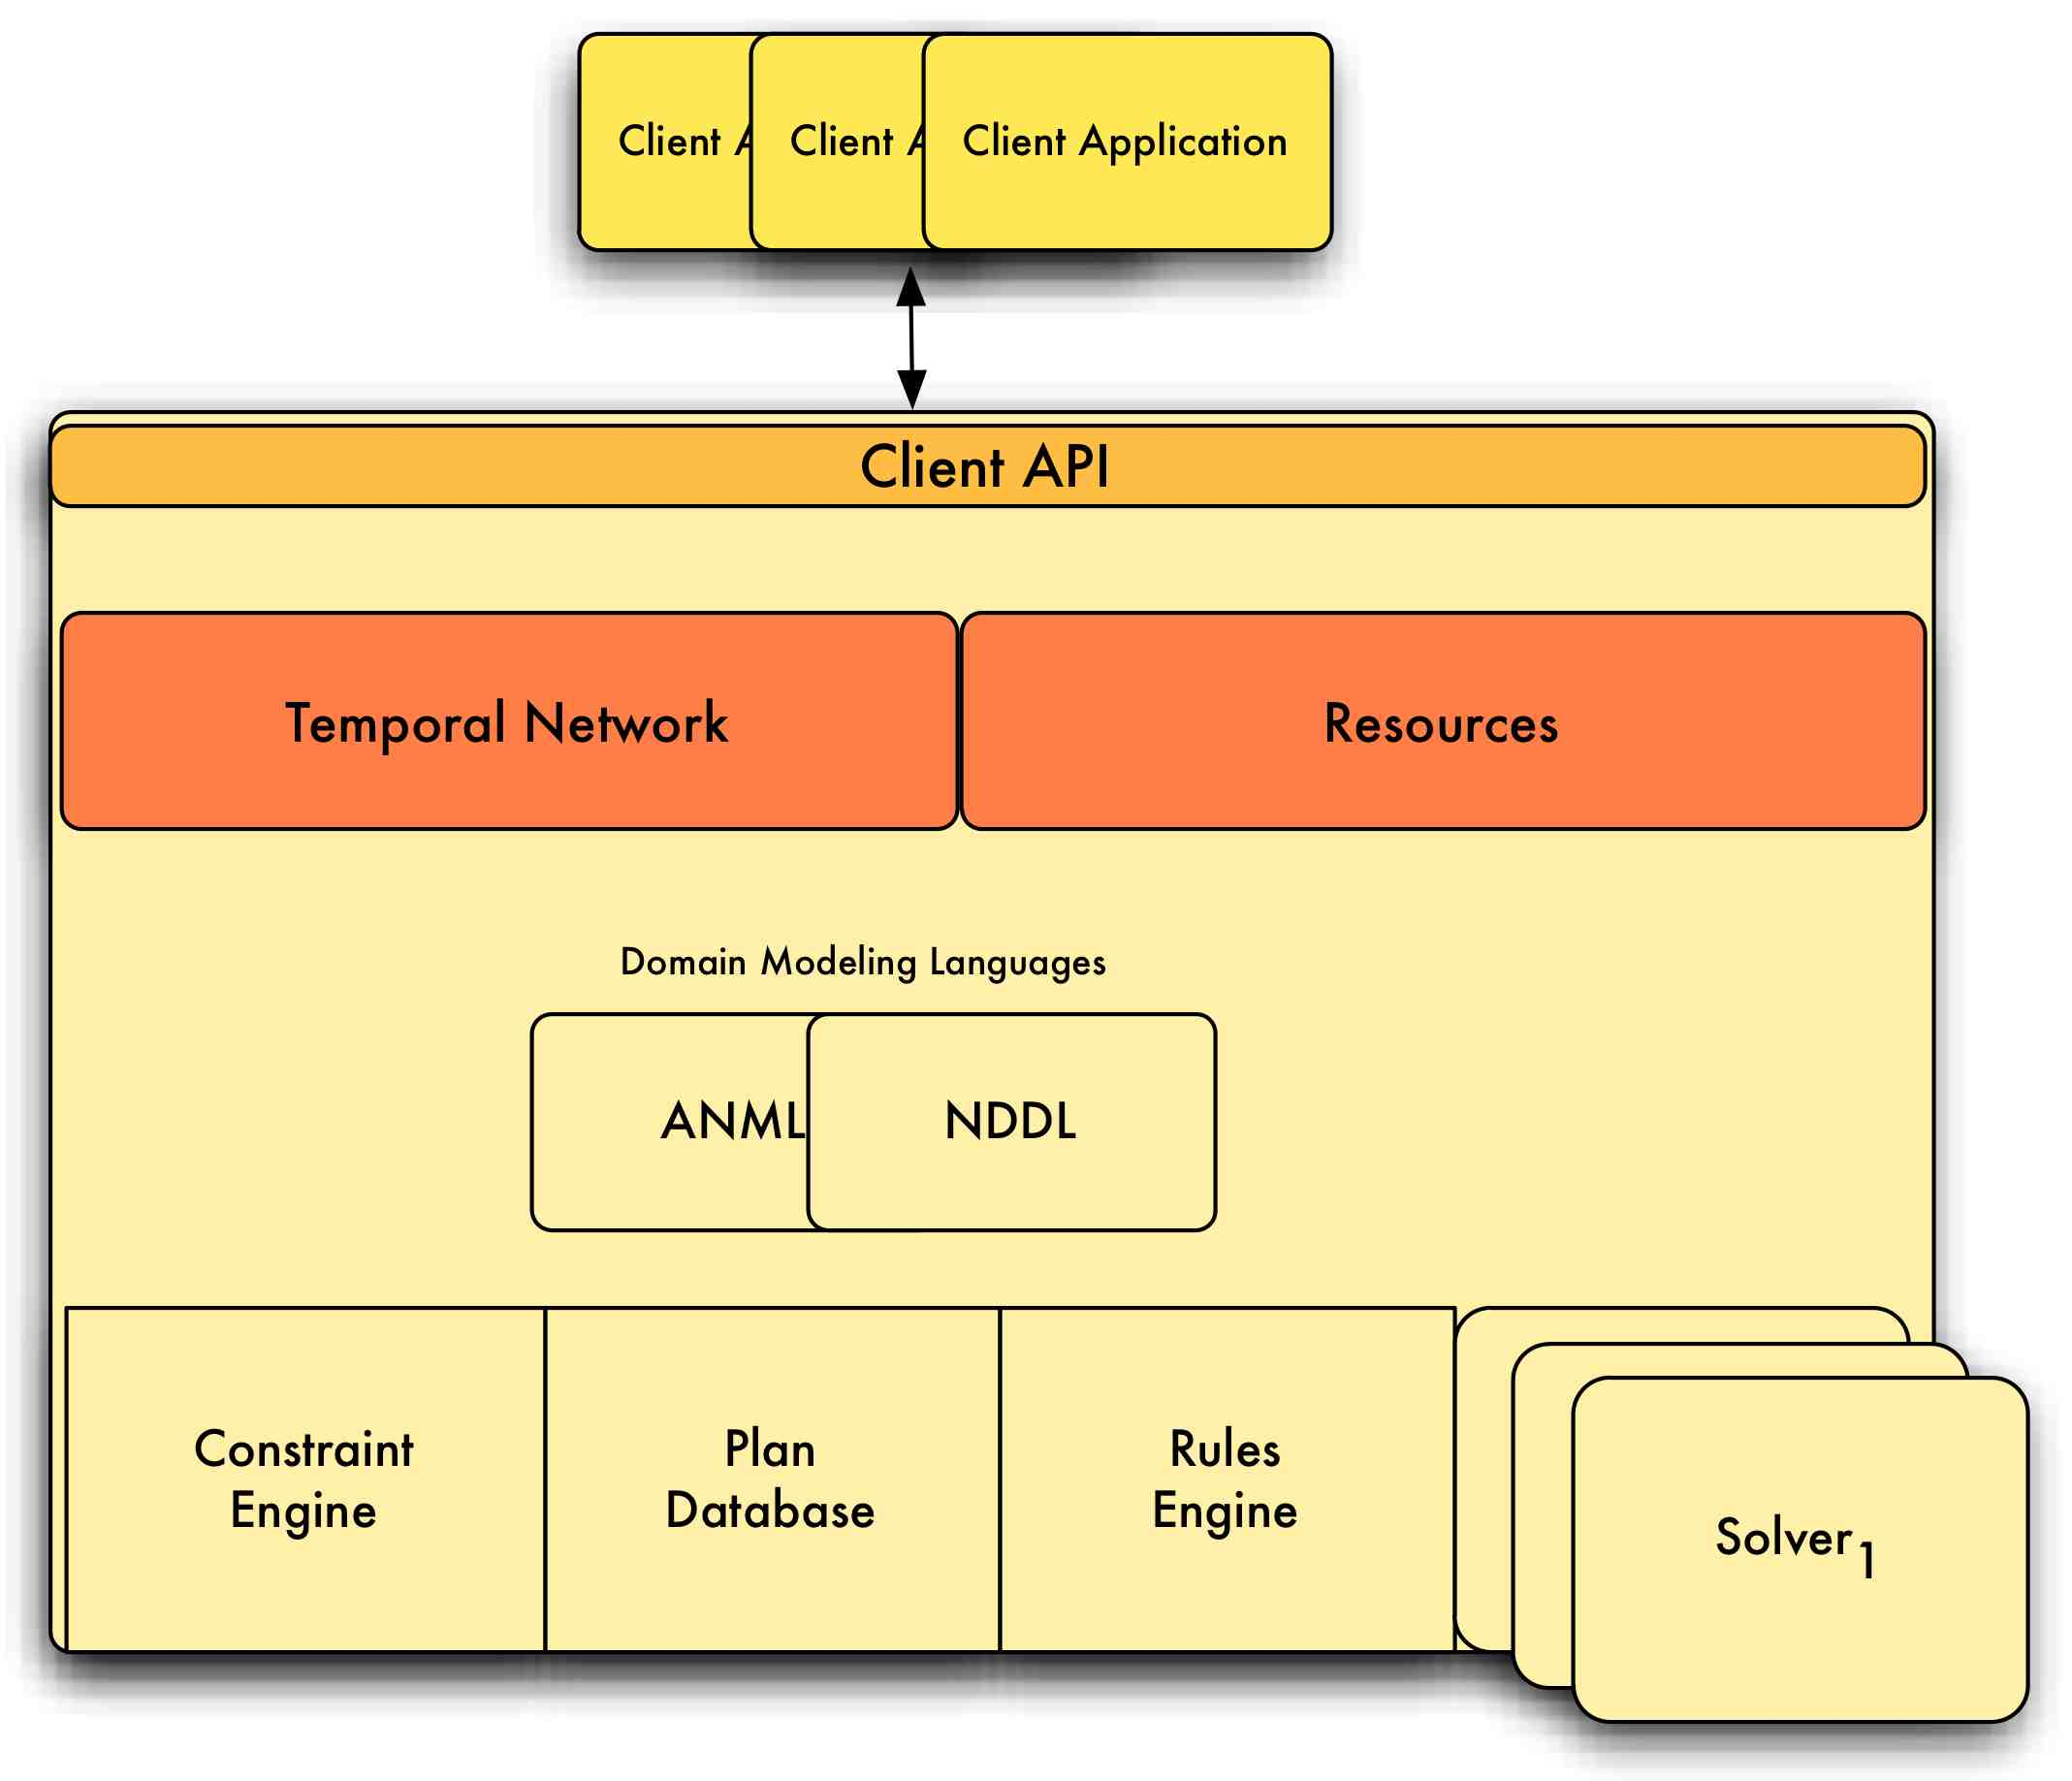
\includegraphics[scale=0.5]{figs/EUROPA-Architecture.jpg}
\caption{\small The \eu Architecture}
\label{fig:europa-architecture}
\vskip+0.1cm
\end{figure}

Fig. \ref{fig:europa-architecture} shows the main architectural
components in \eu and their relationships. 

The \textbf{Constraint Reasoning Engine} (CRE) manages domain types,
variables and constraints that define relationships among them. It
also provides an efficient arc consistency mechanism
\cite{mackworth77}. The CRE is designed so that specialized reasoning
algorithms for specific constraints can be easily and efficiently
plugged in.

The \textbf{Plan Database} (PDB) manages object and token types. It
also maintains the state of partial plans in terms of object, variable
and token instances. This constitutes the data foundation on which end
user applications and automated planners are built.

The \textbf{Rules Engine} (RE) modularly adds the capability to
support domain rules that describe dependencies between tokens,

The \textbf{Solver Module} provides the framework for flaw detection
and resolution that is needed to implement search algorithms for
planning.

The \textbf {Language Modules}: Describing problem domains and problem
instances in terms of objects, variables and domain rules in a
programmatic way is cumbersome to the extent of being impractical,
that motivated the creation of modeling languages that support those
definitions in a much more natural and compact way. NDDL is the main
modeling language for \eu and will be described in detail in the
Modeling section below. ANML is a language under development that
provides a more intuitive syntax \cite{smith08}.
  
The \textbf{API Layer} provides access to services from all the
different modules in a programmatic way so that \eu can be easily
embedded into specialized applications.

 
In an effort to mimimize the amount of work that a user needs to
perform to solve specific problems, \eu also provides extension
modules that have been found to be useful in many domains:

\begin{enumerate}

\item \textit{Temporal Network}: Extensions to the CRE module to
  reason about temporal constraints

\item \textit{Resources}: Extensions to the CRE, PDB and Solver
  modules to provide out-of-the-box reasoning and search for metric
  resources.

\item \textit{Chronological Backtracking Solver}: A general purpose
  built-in solver to provide the ability to plan out-of-the-box,
  problems that require challenging search may require specialized
  solvers to be built as explained in the Search section below.
\end{enumerate}

\subsection{Modeling}
\label{sec:europa:modeling}

\eu can ingest descriptions of models, plans and goals and thereby can
be applied to different domains and problems, simply by providing
different models and goals. Consequently the expressiveness of the
language for models, goals and plans is of great importance. For \eu,
NDDL (New Domain Description Language [pronounced ``noodle''] allows
the user to specify the different components of a problem domain in a
concise way. The main characteristics that make NDDL a powerful tool
for describing problem domains are:

\begin{enumerate} 

\item Object Oriented: NDDL supports classes and inheritance in
  similar fashion to popular Object-Oriented languages like Java and
  C++. It also supports polymorphism for some of the planning
  components. Using object classes and instances is a time-tested
  approach to naturally describe problem domains \comment{OO
    citation}.

\item It offers declarative constructs to define constraints and
  causality dependencies between actions and effects.

\item It offers procedural constructs to populate \eu's plan database
  with specific problem instances expressed in terms of objects,
  variables, constraints, facts and goals.

\end{enumerate}

To understand how the most important elements of NDDL work, we show
how the Shopping Agent problem could be modeled:

\begin{verbatim}

// Locations (Home, SuperMarket, etc.)
class Location {
  string name;
  Location(string _name){
    name = _name;
  }
}

// Products (Milk, Banana, etc.) and
class Product {
  string name;
  Product(string _name) {
    name = _name;
  }
}

// ProductLocations (Banana can be found at SuperMarket, for example)
class ProductLocation {
  Location location;
  Product product;

  ProductLocation(Location _location, Product _product){
    location = _location;
    product = _product;
  }
}

// Use built-in Timeline functionality to enforce that an agent:
// a) Can't be at more than one place at a time.
// b) Can't Go more than one place at a time.
// c) Can't Go somewhere and be At somewhere at the same time.
class AgentLocation extends Timeline{
  predicate At {
    Location loc;
  }

  predicate Going {
    Location from;
    Location to;
  }
}

// In addition to having a location timeline, the agent can buy and own things.  
// Note that the actions and the location predicates can be concurrent 
// so they can't be on the same Timeline
class Agent {
  AgentLocation location;

  Agent() {
    location = new AgentLocation();
  }

  action Buy {
    Product product;
  }
  
  action Go {
    Location from;
    Location to;
  }
  
  predicate Own {
  	Product product;
  }
}
\end{verbatim}

In the model above we can see how the main elements or a problem
domain can be mapped to \eu's representation:

\begin{enumerate}

\item \textbf{Object Types}: NDDL supports an object-oriented
  approach, where common data and behavior can be abstracted as a
  class. In this case, we have the \textit{Product} class represent
  the products that the Shopping Agent needs, \textit{Location}
  represents the places where products can be found,
  \textit{ProductLocation} represents the association arising when a
  product can be purchased at a location. The Shopping Agent itself is
  represented by an \textit{Agent} class, which relies on the
  \textit{AgentLocation} class to keep track of where the agent is at
  any point in time. NDDL supports a single rooted class hierarchy so
  that state and behavior can be extended through inheritance. We took
  advantage of that by making \textit{AgentLocation} inherit from
  \eu's built-in \textit{Timeline} class which doesn't allow
  predicates to overlap in time for the same object instance, in this
  way we can ensure that and agent can only be at one place at a time.

\item \textbf{Variable Types and Instances} : All object attributes
  are represented as variables in this model, for instance, it uses
  integer variables to represent the built-in temporal parameters for
  each token (activity duration, start and end times), string
  variables to represent \textit{Location} and \textit{Product} names,
  and object reference variables to represent the structural
  relationships between different objects (for instance, each Agent
  has variable to keep track of its \textit{AgentLocation}).

\item \textbf{Predicate Types}: Some classes like \textit{Product},
  \textit{Location} and \textit{ProductLocation} are completely static
  and so don't have any predicate or action types associated with
  them. The \textit{AgentLocation} class is purely used to keep track
  of state and so it has \texttt{At} and \texttt{Going} predicate
  types associated with it. The \textit{Agent} class keeps track of
  the products it purchases through the \texttt{Own} predicate, having
  a separate \textit{AgentBag} class with its own predicates would
  have been an equally valid modeling choice.

\item \textbf{Action Types}: The \textit{Agent} class is the only one
  that has behavior associated with it, consequently, it defines
  action types to represent when the agent is taking action to
  \texttt{Go} to a \textit{Location}, or to \texttt{Buy} a
  \textit{Product}. We'll see how the actual behavior for those
  actions is specified below.
\end{enumerate}

\begin{verbatim}

// Define the rules for our actions:
Agent::Go {
  met_by(condition object.location.At origin);
  eq(from, origin.loc);
 
  equals(effect object.location.Going going);
  eq(going.from, from);
  eq(going.to, to);
   
  meets(effect object.location.At destination);
  eq(to, destination.loc);
}

Agent::Buy {
  // A Buy takes 10 time units
  eq(10, duration);

  // initialized to all locations
  ProductLocation possibleStores;

  // limit possibleStores variables to ones that provide what we need to buy
  eq(product, possibleStores.product);

  // We must be At a location during our Buy, and that location must have the
  // product we want available:
  contained_by(condition object.location.At currLocation);
  eq(currLocation.loc, possibleStores.location);
  
  starts(effect Own purchase);
  eq(purchase.product,product);
}
\end{verbatim}

Domain rules can be defined in NDDL in the context of a Predicate or
an Action. In the example above we can see the main elements of a rule
definition:

\begin{enumerate}
\item \textbf{Variables}: A Token Type (predicate or action) is part
  of a class, therefore class attributes (see references to
  \texttt{object.location} above), Token Type parameters (see
  references to \texttt{[from, to]} in \texttt{Agent::Go}, or to
  \texttt{[duration, product]} in \texttt{Agent::Buy} and locally
  declared variables (see \texttt{possibleStores} in
  \texttt{Agent::Buy}) can all be used in the definition of a Rule.

\item \textbf{Constraints}: restrictions on the values that variables
  can take inside a Rule are expressed through constraints, in the
  example above only the \texttt{eq} constraint is used, but in
  general, any constraint available in \eu's library can be used.

  \item \textbf{Subgoals}: In \texttt{Agent::Go}, subgoals are used to
    specify that the Shopping Agent's location must transition from
    origin to destination in a temporally consistent way. The
    \texttt{[meets, equals, metby]} operators are used to specify
    subgoals (Allen operators are explained in more detail below),
    along with the temporal relationship each token representing a
    subgoal has with the the token representing the \texttt{Agent::Go}
    action. Also, \texttt{[condition, effect]} annotations can be used
    when defining a subgoal inside an action, \eu doesn't immediately
    associate any semantics with them, but they can be extremely
    useful for search modules when creating plans.
\end{enumerate}

Now, having that we have a specification for the Shopping Agent
domain, here is how a particular problem instance could be specified:

\begin{verbatim}

// Allocate instances
Location Home = new Location("Home");
Location SuperMarket = new Location("SuperMarket");
Location HardwareStore = new Location("HardwareStore");

Product Banana = new Product("Banana");
Product Milk = new Product("Milk");
Product Drill = new Product("Drill");

ProductLocation bananaLocation = new ProductLocation(SuperMarket, Banana);
ProductLocation milkLocation = new ProductLocation(SuperMarket, Milk);
ProductLocation drillLocation = new ProductLocation(HardwareStore, Drill);

Agent agent = new Agent();

// Indicate that the database is closed - no new objects can be created
// this allows EUROPA to perform more efficient inference
close();

// We start the day at Home:
fact(agent.location.At atHomeForBreakfast);
atHomeForBreakfast.loc.specify(Home);

// Goals for all of the agent's needs, buy if needed
goal(agent.Own gotMilk);
gotMilk.product.specify(Milk);
goal(agent.Own gotBanana);
gotBanana.product.specify(Banana);
goal(agent.Own gotDrill);
gotDrill.product.specify(Drill);

// Make sure agent is home for dinner
goal(agent.location.At atHomeForDinner);
atHomeForDinner.loc.specify(Home);

// Agent has all day to satisfy goals:
gotMilk after atHomeForBreakfast;
gotMilk before atHomeForDinner;

gotBanana after atHomeForBreakfast;
gotBanana before atHomeForDinner;

gotDrill after atHomeForBreakfast;
gotDrill before atHomeForDinner;

// Force things to happen within our planning horizon:
int horizonStart = 0;
int horizonEnd = 100;
leq(horizonStart, atHomeForBreakfast.start);
leq(atHomeForDinner.end, horizonEnd);

\label{eu:model}
%\caption{Specifying a problem instance for the Shopping Agent in NDDL}
\end{verbatim}

A problem instance consists mainly of 

\begin{enumerate}

\item \textbf{Variables} and \textbf{Objects}: In this case we defined
  temporal variables that are used to specify the planning horizon
  (see \texttt{horizonStart} and \texttt{horizonEnd}), and objects are
  used to specify the locations, products, product-location
  associations and the Shopping Agent that we want to plan for.

\item \textbf{Facts}: These are used to specify the current state of
  the world and don't need any support. Facts are represented as
  tokens in \eu's Plan Database. In this case we use facts to specify
  that the Shipping Agent is initially at home.

\item \textbf{Goals}: Goals are represented as tokens in \eu's Plan
  Database, differently from Facts, Goals trigger inference in \eu
  which determines whether flaws (unresolved subgoals, overloaded
  resources, etc., flaws will be covered in detail in the search
  section below) need to be resolved, if that is the case, search
  modules can be invoked which will look for a plan where all the
  flaws are resolved.

\item \textbf{Constraints}: restrictions on and between actions and
  goals are specified through constraints, in this case we use
  temporal constraints to specify when the facts hold and when the
  goals should be accomplished. As always, all the constraints in
  \eu's library (built-in, or user defined), can be used to specify
  these restrictions.
\end{enumerate}


\subsection{Inference}
\label{sec:europa:inference}

\comment{explain how inference is used to detect perform bounds
  propagation, domain reduction and to detect constraint violations.} 
- talk about AC3 implementation and extension mechanisms
- talk about europa's constraint library


The Temporal Network: The notion of time is central to temporal
planning. \eu uses variables to explicitly represent timepoints for
plan activities and states. Constraints among timepoints provide a
natural way to express domain axioms. For example, in order to state
that activity A must occur before activity B we can say that the end
timepoint of A is $leq$ the start timepoint of B.

\begin{figure}
\centering
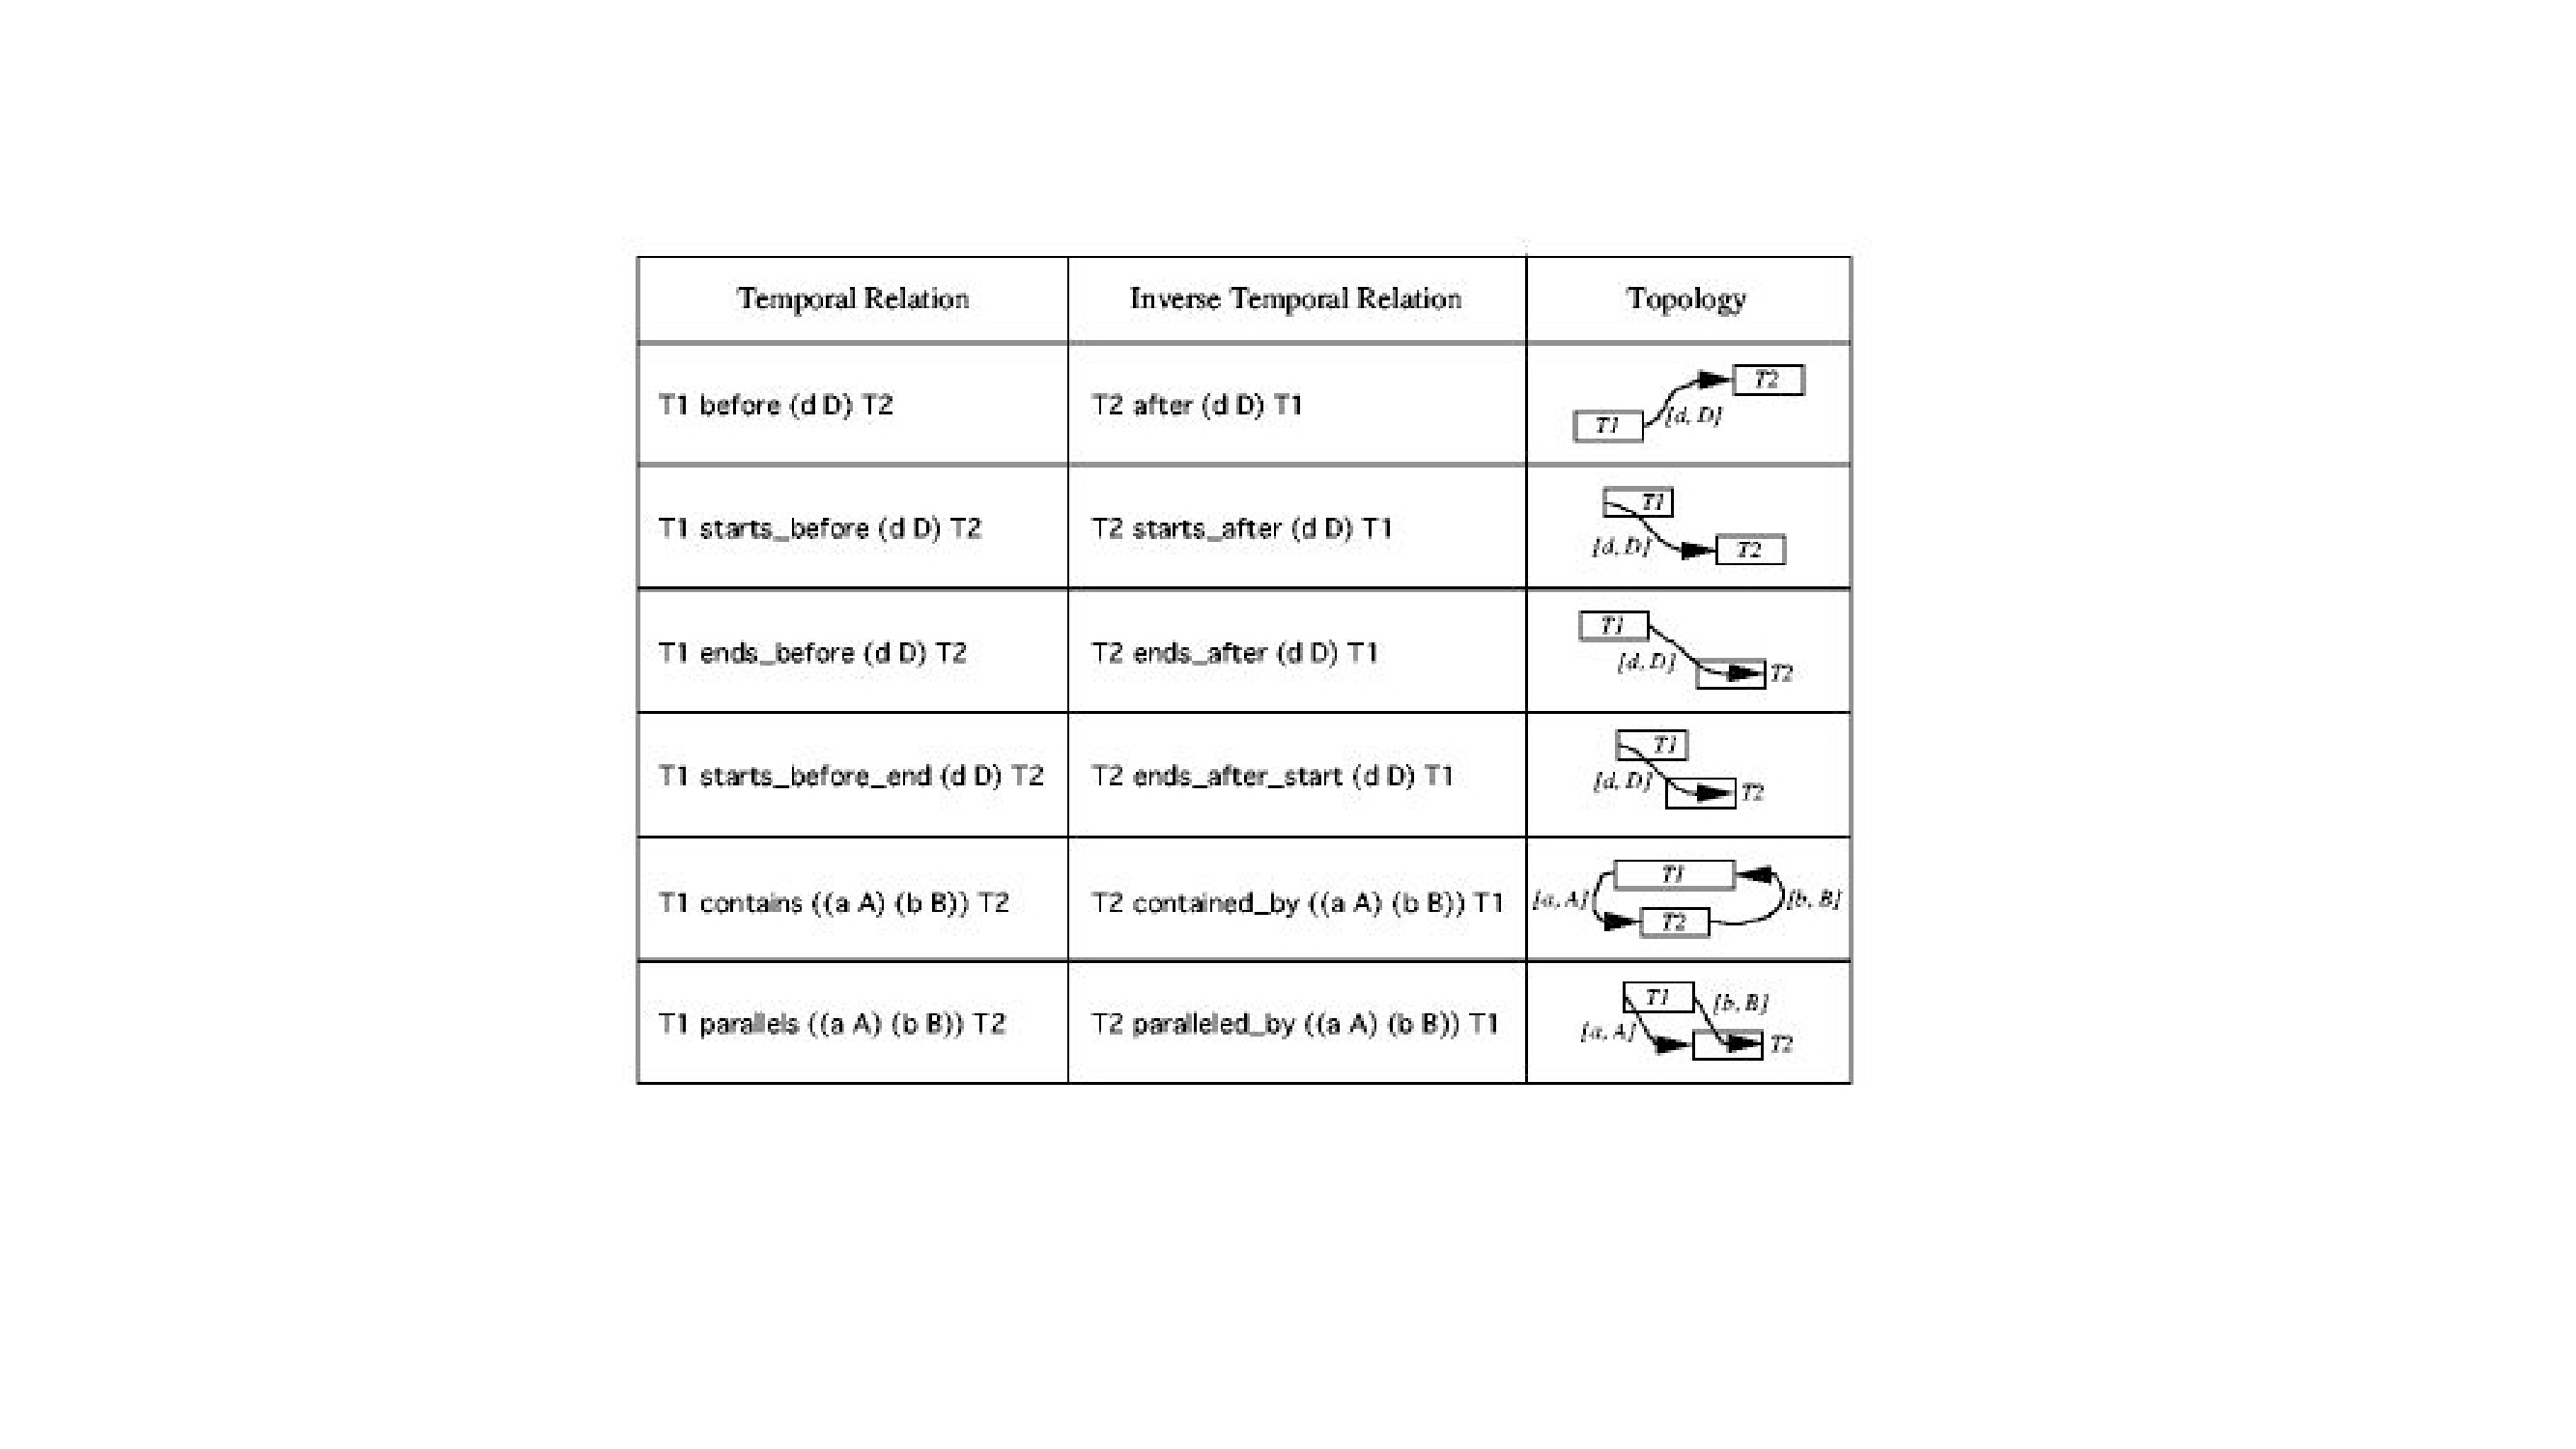
\includegraphics[scale=0.3]{figs/Allen-algebra.pdf}
\caption{\small Temporal relations defined within the planner are
  based on \texttt{Allen Algebra} relations shown above.}
\label{fig:allen-algebra}
\vskip-0.3cm
\end{figure}

\cite{dechter91} proposed that constraints among timepoints can be
grouped together to form a Simple Temporal Network (STN). Such a
network can be transformed into a Distance Graph (DG) where the
outward arc from a node represents the maximum distance from the
source node to the target node. They also showed that shortest path
algorithms could be used to propagate values in the network and
discover a negative cycle. A negative cycle is a path from a node to
itself that has a path length less than 0. If such a cycle exists, the
network is inconsistent. It was further shown that a single-source
shortest path algorithm was sufficient to detect a negative cycle and
provide sufficient propagation to yield a backtrack-free search. Thus
we have an efficient and complete algorithm for propagating an
STN. These results build on the already established notion of a CSP
and are naturally incorporated into the general representation and
propagation scheme used in \eu.  The diagram below illustrates a
simple STN with just 2 variables and a single constraint. It also
shows the resulting DG.


\begin{figure}[!htb]
  \centering
  \subfloat[\small A Simple Temporal Network (STN)]{\label{fig:stn1}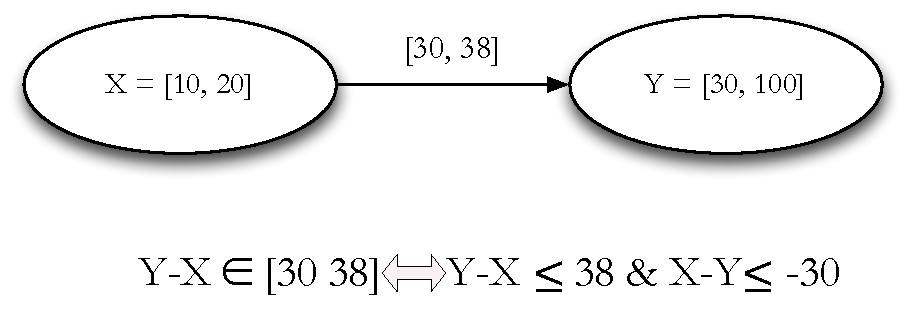
\includegraphics[width=0.4\columnwidth]{figs/stn-graph.pdf}}
  \subfloat[\small Resulting distance graph from \ref{fig:stn1}.]{\label{fig:stn2}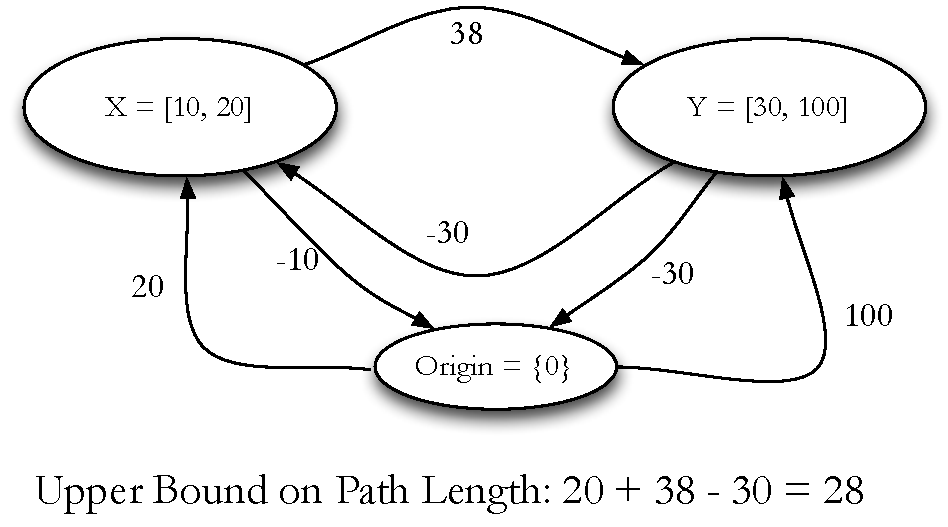
\includegraphics[width=0.4\columnwidth]{figs/distance-graph.pdf}}
    \caption{\small An illustration of a STN and its corresponding
      distance graph.}
  \label{fig:stn}
\end{figure}

% \comment{ add figure. Use Europa wiki figure; or use conor figure from slides}


Resources:

\begin{enumerate}

\item \textbf{Reservoir} resources can have both 'consume' and
  'produce' tokens. Note that these tokens do NOT have the usual
  start/end/duration token variables, since occur at a single instant
  in time. Instead, they have a single variable, 'time' used to
  represent that instant.

\item \textbf{Reusable} resources have 'uses' tokens that use a
  quantity for the duration of the token. These tokens do have the
  usual start/end/duration variables.

\item \textbf {Unary} resources are reusable resources with unit
  quantity and have 'use' tokens (again, with the usual
  start/end/duration variables).
\end{enumerate}

\comment{talk about resource envelope computation by using MaxFlow formulation.}


\subsection{Search}
\label{sec:europa:search}

Now we have all the elements in place so that an automated problem
solver can be created. Let's recap what those elements are:

\begin{enumerate}

\item A domain model that describes the variable, object, predicate
  and action types that are relevant for the problem.

\item A problem instance (also called initial state) that consists of:
\item Variable and Object instances that exist for the entire planning
  horizon.
\item Temporally scoped predicate and action instances.
\item Temporally scoped goals.

\end{enumerate}
	
This information is kept in \eus Plan Database so that inference and
search mechanisms can be used to look for a problem solution.

Given that temporal intervals may extend indefinitely in both positive
and negative directions, for problems with a temporal dimension it is
also common to specify a Planning Horizon when invoking a solver. The
Planning Horizon is the temporal interval that a problem solver has to
worry about, any decisions that fall completely outside of the
Planning Horizon can be ignored. This is very useful for recurrent
activities, consider for instance a model where a medical checkup has
to occur every 3 months, the user can model a recurring activity and
then use the Planning Horizon to ensure that a finite number of
medical checkup activities are generated as part of a plan. This is
also useful to ignore activities that may happen too far in the future
or in the past to be relevant for a particular plan, this way the user
can ensure that the solver is making as few commitments as necessary.

\eu provides a built-in solver that performs Plan Space Planning
\cite{ghallab04} in this approach, the initial state is considered a
partial plan that needs to be refined toward a solution plan that
achieves the goals. The operations to refine the partial plan PP at
any time are:

\begin{enumerate}
\item Find the flaws of PP, that is the conditions that prevent it
  from being a solution plan (flaw types are explained below).
\item Select one such flaw
\item Select a resolver for the flaw
\item Refine PP by applying the resolver
\item If an inconsistency is found, try another resolver.
\item If all possible resolvers for a particular flaw fail, return
  failure, otherwise continue until resolving all the flaws.
\end{enumerate}
	
This Plan Space Planning algorithm is translated into \eu's
representation as follows:

The initial partial plan is the state of \eus Plan Database after the
initial state has been instantiated, this results in a set of
variable, object and token instances. Inference then takes place to
detect flaws in the partial plan, there are 3 kinds of flaws that can
be detected:

\begin{enumerate}

\item Unbound Variable: a variable in the partial plan whose domain is
  not a singleton. Unbound Variables are resolved by specification of
  a value from the domain of the variable.

\item Open Condition: an open condition is an inactive token. Inactive
  tokens can be generated by explicitly posted goals, or when a token
  is activated, rules may fire that create inactive slave tokens
  \comment{point to more detailed decription above in Rules Engine
    section}.  Open Conditions can be resolved in three ways:

  \begin{enumerate}

  \item Merging: A free activity is merged with a matching activity
    already in the plan. An activity a is said to match an activity a?
    if a and a? unify and the temporal constraints involving a are
    satis�ed by a?. Thus, a and a? can be considered the same activity
    and we do not need to introduce a in the plan. Consequently, the
    compatibilities associated with a are not �red, because they have
    been already triggered when a? was introduced in the plan.

  \item Activation: We introduce a new activity a in the current plan
    associating it with the proper timeline, but without choosing a
    speci�c time slot for it.The compatibilities associated with a are
    applied and the subgoal activities resulting from those
    compatibilities are introduced as free activities. This results in
    both an ordering flaw, corresponding to the just activated activity,
    and a number of open condition flaws, corresponding to the new
    subgoal activities.

  \item Rejection: Some goals may be optional, if that is the case for a
    particular order condition, its corresponding flaw can be resolved
    by discarding the inactive token. 

\end{enumerate}

\item Threat: once a token has been placed in the partial plan it may
  impact other tokens indirectly through possible overlapping
  requirements on objects. Recall for example that a token may belong
  to objects (e.g. Timelines) which require a total order over their
  tokens. If any 2 tokens could possibly overlap (though not
  necessarily), then they pose a threat to each other in terms of
  achieving an extension of the current partial plan which is complete
  and consistent. Similarly, threats may arise where tokens share a
  common resource and their current state might yield extensions of
  the current partial plan which are inconsistent. Threats are
  resolved by imposing ordering constraints among tokens.

\end{enumerate}

Open Conditions and Threats allow flaw detection and resolution at a
higher-level of abstraction (i.e. in terms of objects and tokens) than
that of simply binding variables as is common in Constraint
Satisfaction Problems. This is advantageous when one applies
heuristics for ordering choices since it provides a richer context in
which to make decisions.  Furthermore, it aids in reducing the amount
of work done by a solver so that only the necessary refinements are
made, otherwise leaving the partial plan with maximum flexibility. For
example, one can omit unbound variables which are time-points of
tokens since threats will force a solver to impose restrictions on
these variables based on the semantics of the objects to which their
tokens apply. Thus the planning process may yield partially-ordered
plans for which all possible extensions are provably valid.

The Plan Space Planning algorithm described above can be implemented
in many different ways depending on the approach chosen for flaw and
resolver selection and for backtracking. \eus built-in solver
implements a chronological backtracking algorithm that is summarized
in Algorithm \ref{alg:europa:solve}.


\begin{algorithm}[H]
\KwIn{PartialPlan $plan$}
\KwOut{\texttt{true} if a plan solution was found, \texttt{false} otherwise}
\Begin{
  \lIf{isInconsistent(plan)}{\Return \texttt{false}\;}\label{li:propagate}
  \BlankLine
  Flaw $flaw \leftarrow chooseFlaw(plan)$ \; \label{li:selectflaw}
  \lIf{ $\emptyset = flaw$ }{\Return \texttt{true} \;} \label{li:noflaw}
  \BlankLine
  DecisionPoint $decision \leftarrow makeDecisionPoint(flaw, plan)$ \; \label{li:decisionpt}
  \While{ $decision.hasNext()$ }{ \label{li:decisionloop}
    PartialPlan $pp \leftarrow decision.executeNext()$ \; \label{li:decide}
    \lIf{ $solve(pp)$ }{ \Return \texttt{true} \; } \label{li:recurse}
    \lElse{ $decision.undo()$ \; } \label{li:backtrack}
   }
   \Return \texttt{false} \; \label{li:noplan}
 }
\caption{$\mathrm{bool} ~ solve(plan)$}
\label{alg:europa:solve}
\end{algorithm}


The algorithm takes as input a partial plan p and returns true if a
complete and consistent refinement of p could be found (or if p is
initially complete and consistent), and false otherwise.

\begin{enumerate}

\item Line \ref{li:propagate}: Propagate the constraints to test for
  inconsistency. If found to be inconsistent, then we can return false
  since this is a dead-end i.e. no refinements to p can yield a
  consistent plan.

\item Line \ref{li:selectflaw}: Choose a flaw from the set of
  available flaws.

\item Line \ref{li:noflaw}: If there are no flaws, then p is complete
  and we can terminate with success.

\item Line \ref{li:decisionpt}: Otherwise we formulate a decision
  point which is a branch in the search space. Each choice is a
  particular refinement operation and the DecisionPoint collects all
  possible refinement operations for the given flaw.

\item Line \ref{li:decisionloop}: We keep trying until the chosen flaw
  is resolved, or until we run out of resolvers to try.

\item Line \ref{li:decide}: A new partial plan is obtained by
  application of a refinement operator. Note that the ordering over
  refinement operators to select is a non-deterministic step.

\item Line \ref{li:recurse}: Recursive call to solve the new planning
  problem. If successful, then we are done.

\item Line \ref{li:backtrack}: Otherwise, retract the last refinement
  operation and move on to try the next one.

\item Line \ref{li:noplan}: If we arrive here, then we have exhausted
  all options to resolve the flaw, including the case where no options
  were available initially. Thus the problem cannot be solved.
\end{enumerate}


This algorithm provides for a sound and complete search, assuming that
no flaws or available refinement operators are pruned unnecessarily.
Dead-ends in the search are discovered through constraint propagation.
Constraint propagation is a vehicle for evaluating the consistency of
a partial plan and also for filtering infeasible values from
consideration prior to commitment, allowing in some cases a strong
look-ahead capability which is essential for tractable
search. Consistency testing is initiated by the isConsistent
procedure. The algorithm permits a heuristically controlled search by
applying orderings for chooseFlaw and makeDecisionPoint. It results in
a chronologically-backtracking search.

\comment{expand a little more on how heuristics can be implemented by
  applying ordering/filtering for chooseFlaw and makeDecisionPoint}
examples:
- deal with earliest flaws first
- deal with planning (open condition flaws) before scheduling (threats) ones

It should be emphasized that while this algorithm is commonly
employed, it is only one of many that could be
implemented. \comment{give examples of local search solvers for
  scheduling and CSP?}

N-Queens solver:
\begin{verbatim}
    public void solve(int maxIter)
    {
    	init();
    	
    	for (int i=0;psengine_.getViolation() > 0 && i < maxIter;i++) {
    	    PSVariable queenToMove = getQueenWithMaxViolation();
    		int curPos = queenToMove.getSingletonValue().asInt();
    	    
    	    boolean moved = false;
            SortedSet<Move> moves = getMoves(queenToMove,curPos);             
            for (Move m : moves) {
            	moved = makeMove(queenToMove,curPos,m,false);
            	if (moved)
            	    break;
            }
            
            if (!moved) 
            	makeMove(queenToMove,curPos,moves.first(),true);
            
            checkSolution(); // See if we have a new best solution            
            notifyIterationCompleted(curIteration_++);
            
            if (curIteration_-bestIter_ > 50) 
            	restart();
    	}
    }
\end{verbatim}

RCPSP solver \comment{Do we need this example?}:
\begin{verbatim}
    public void solve(PSEngine psengine,
    		          long timeout, // in msecs
    		          int bound)
    {
       init(psengine,timeout,bound);
       
       for (int i=0; true ; i++) {
          flatten();
          updateSolution(i);
          updateCriticalPrecedences();
          
          if ((nbStable_ > maxStable_) || (bestMakespan_ <= makespanBound_))
             break;
          
          if (timer_.getElapsed() > timeout) {
              timedOut_ = true;
              break;
          }
          
          relax();
          curIteration_++;
       }       

       restoreBestSolution();
    }

\end{verbatim}


\comment{explain how other solvers can be built, maybe use NQueens or
  RCPSP example to illustrate. Or maybe build a little specialized
  solver for shopping or rover examples.}


%%% Local Variables: 
%%% mode: latex
%%% TeX-master: "setobook"
%%% End: 


 